\documentclass{article}
\usepackage{tikz}

\begin{document}

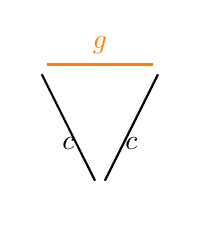
\begin{tikzpicture}[scale=0.8]
    % Nodes
    \node (A) at (0,0) {};
    \node (B) at (2,0) {};
    \node (C) at (1,-2) {};

    % Edges
    \draw[thick, orange] (A) -- node[midway, above] {$g$} (B);
    \draw[thick, black] (A) -- node[midway, below] {$c$} (C);
    \draw[thick, black] (B) -- node[midway, below] {$c$} (C);

    % Labels for nodes if needed
    % \node at (A) [below left] {Node A};
    % \node at (B) [below right] {Node B};
    % \node at (C) [above] {Node C};

\end{tikzpicture}

\end{document}